\documentclass{article}\usepackage[]{graphicx}\usepackage[]{color}
%% maxwidth is the original width if it is less than linewidth
%% otherwise use linewidth (to make sure the graphics do not exceed the margin)
\makeatletter
\def\maxwidth{ %
  \ifdim\Gin@nat@width>\linewidth
    \linewidth
  \else
    \Gin@nat@width
  \fi
}
\makeatother

\definecolor{fgcolor}{rgb}{0.345, 0.345, 0.345}
\newcommand{\hlnum}[1]{\textcolor[rgb]{0.686,0.059,0.569}{#1}}%
\newcommand{\hlstr}[1]{\textcolor[rgb]{0.192,0.494,0.8}{#1}}%
\newcommand{\hlcom}[1]{\textcolor[rgb]{0.678,0.584,0.686}{\textit{#1}}}%
\newcommand{\hlopt}[1]{\textcolor[rgb]{0,0,0}{#1}}%
\newcommand{\hlstd}[1]{\textcolor[rgb]{0.345,0.345,0.345}{#1}}%
\newcommand{\hlkwa}[1]{\textcolor[rgb]{0.161,0.373,0.58}{\textbf{#1}}}%
\newcommand{\hlkwb}[1]{\textcolor[rgb]{0.69,0.353,0.396}{#1}}%
\newcommand{\hlkwc}[1]{\textcolor[rgb]{0.333,0.667,0.333}{#1}}%
\newcommand{\hlkwd}[1]{\textcolor[rgb]{0.737,0.353,0.396}{\textbf{#1}}}%

\usepackage{framed}
\makeatletter
\newenvironment{kframe}{%
 \def\at@end@of@kframe{}%
 \ifinner\ifhmode%
  \def\at@end@of@kframe{\end{minipage}}%
  \begin{minipage}{\columnwidth}%
 \fi\fi%
 \def\FrameCommand##1{\hskip\@totalleftmargin \hskip-\fboxsep
 \colorbox{shadecolor}{##1}\hskip-\fboxsep
     % There is no \\@totalrightmargin, so:
     \hskip-\linewidth \hskip-\@totalleftmargin \hskip\columnwidth}%
 \MakeFramed {\advance\hsize-\width
   \@totalleftmargin\z@ \linewidth\hsize
   \@setminipage}}%
 {\par\unskip\endMakeFramed%
 \at@end@of@kframe}
\makeatother

\definecolor{shadecolor}{rgb}{.97, .97, .97}
\definecolor{messagecolor}{rgb}{0, 0, 0}
\definecolor{warningcolor}{rgb}{1, 0, 1}
\definecolor{errorcolor}{rgb}{1, 0, 0}
\newenvironment{knitrout}{}{} % an empty environment to be redefined in TeX

\usepackage{alltt}

% latex packages
\usepackage{graphicx}
\usepackage[margin=0.75in]{geometry}
\usepackage[backend=bibtex]{biblatex}
\addbibresource{refs.bib}

% title information
\title{Simple Regression}
\author{Gaston Sanchez}
\IfFileExists{upquote.sty}{\usepackage{upquote}}{}
\begin{document}
\maketitle



\begin{abstract}
We analyzed the relationship between height and weight of some inviduals from a galaxy far, far away.
\end{abstract}


\section{Introduction}
This is just a minimal example of a simple regression analysis in R. The goal is to practice creating a reproducible report using several tools such as Makefile, R, knitr, Rnw files, plots, etc.

\section{Data}
We curated a data set from the wookieepedia. Current descriptions in the website do not longer contain information about weight.

% latex table generated in R 3.2.3 by xtable 1.8-2 package
% Mon Mar 14 07:54:48 2016
\begin{table}[ht]
\centering
\begin{tabular}{rlrr}
  \hline
 & name & height & weight \\ 
  \hline
1 & Anakin Skywalker & 188 &  84 \\ 
  2 & Padme Amidala & 165 &  45 \\ 
  3 & Luke Skywalker & 172 &  77 \\ 
  4 & Leia Skywalker & 150 &  49 \\ 
  5 & Obi-Wan Kenobi & 182 &  77 \\ 
  6 & Han Solo & 180 &  80 \\ 
  7 & R2-D2 &  96 &  32 \\ 
  8 & C-3PO & 167 &  75 \\ 
  9 & Yoda &  66 &  17 \\ 
  10 & Chewbacca & 228 & 112 \\ 
   \hline
\end{tabular}
\end{table}


There are 10 individuals, with an average height of 159.4 cms, and an average weight of 64.8 kgs. The summary statistics are displayed in the table below:
% latex table generated in R 3.2.3 by xtable 1.8-2 package
% Mon Mar 14 07:54:48 2016
\begin{table}[ht]
\centering
\begin{tabular}{rll}
  \hline
 &     height &     weight \\ 
  \hline
1 & Min.   : 66.0   & Min.   : 17.00   \\ 
  2 & 1st Qu.:153.8   & 1st Qu.: 46.00   \\ 
  3 & Median :169.5   & Median : 76.00   \\ 
  4 & Mean   :159.4   & Mean   : 64.80   \\ 
  5 & 3rd Qu.:181.5   & 3rd Qu.: 79.25   \\ 
  6 & Max.   :228.0   & Max.   :112.00   \\ 
   \hline
\end{tabular}
\end{table}


\subsection{EDA}
We looked at the distributions of height and weight. As suggested by \cite{ductavis}, this relation is almost perfectly linear among human Jedis.

\begin{figure}[h!]
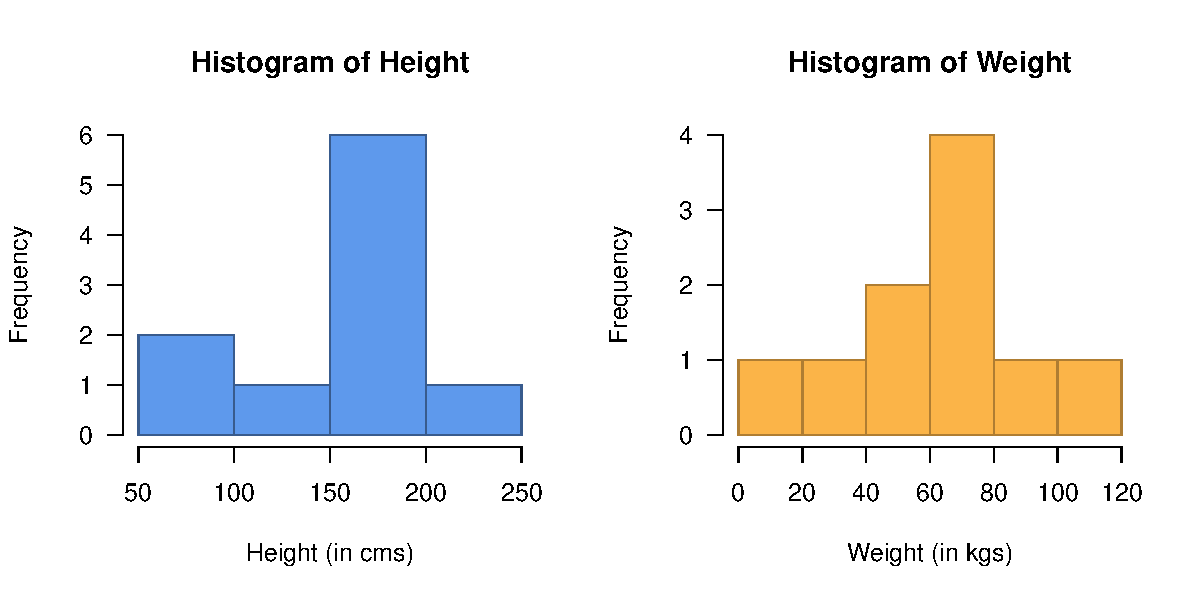
\includegraphics[width=1\textwidth]{../images/histograms.pdf}
\end{figure}

There is a strong linear relationship between height and weight. This is evidenced in the scatterplot, and calculation the correlation 0.9412865.

\begin{figure}[h!]
    \centering
	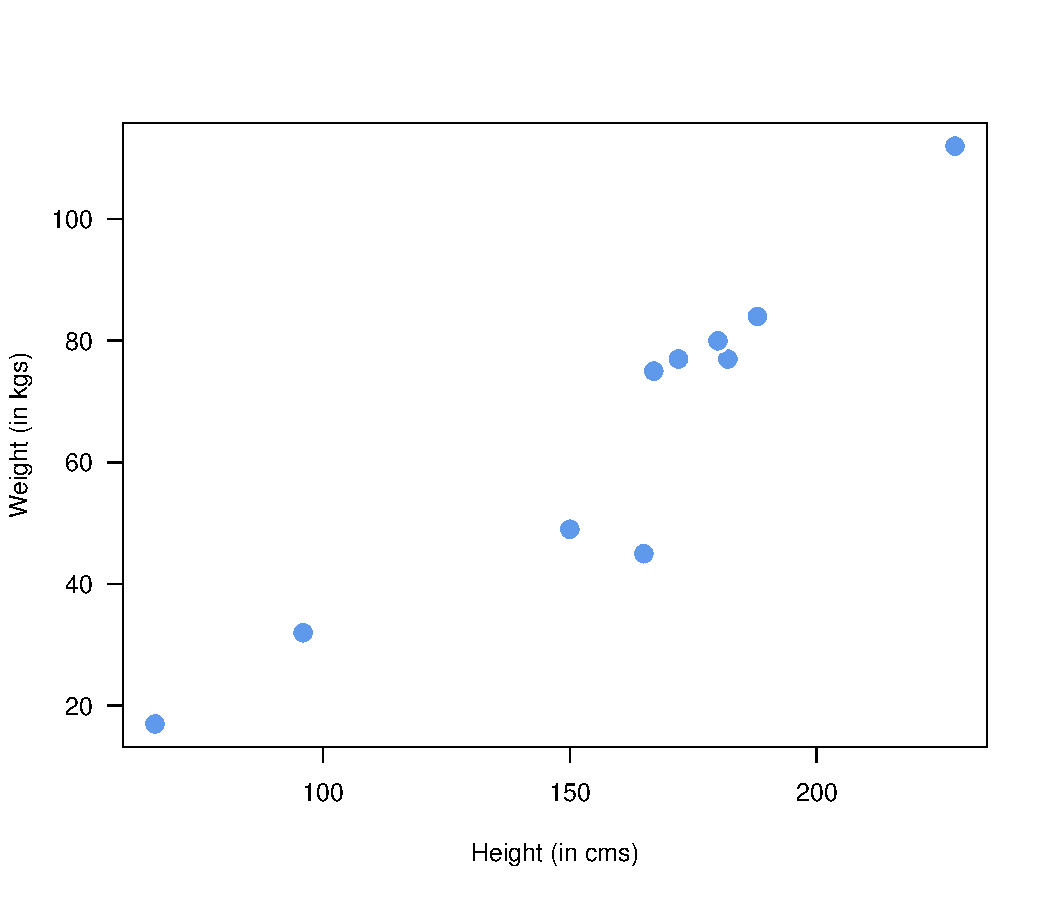
\includegraphics[width=0.9\textwidth]{../images/scatterplot.pdf}
\end{figure}

\section{Conclusions}
Our analysis agrees with Yoda's seminal article \cite{yoda}. But more work needs to be carried out like collecting additional samples in future surveys. May the Force be with you.


\printbibliography
\end{document}
